\chapter{Control system}\label{chap:control_system}
\section{Designing a regulator}
This chapter concerns implementation of a regulator for the pan tilt system. So
far the system has been analyzed as open loop and no feedback has considered.
The objective in designing this controller is to increase the performance of the
system, in this case meaning to track a position. 

\subsection{Requirements}
In the dynamics chapter it was concluded that a decoupled model of the system is
sufficient and therefore a regulator for pan part and a regulator for the tilt
part can be designed individually.

The controller is developed focusing mainly on optimizing the precision and less
on optimizing speed and settling time. Therefore the objective is to design a
regulator with a steady state error of zero. This is in therory done by adding
an integrator, to raise the type of the system, so at least the regulatior should be of type PI.

\subsection{Design}
SISO\footnote{Single input, single output}-control systems can be sketched the
following way:
\begin{figure}[htb]
  \centering
  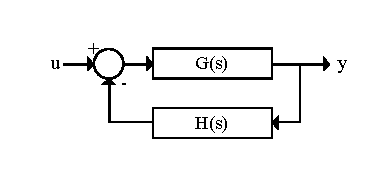
\includegraphics[width=\textwidth,clip,trim=0 10 0 10]{graphics/control_sketch.pdf} %trim=l b r t
	\caption{This figure illustrates a sketch of a general control system.}
	\label{fig:control_sketch}
\end{figure}
Figure \ref{fig:control_sketch} show a system with a feedback loop, $G(s)$ is
the plant and $H(s)$ is the regulator. When designing a regulator ($H(s)$) is
derived and since the system is SISO, a PID regulator can be designed.

\subsection{PID parameters}
A PID regulator can be expressed in the following way:
\begin{equation}
	h(t) = K_p e(t) + K_i \int\limits_0^t e(\tau) d\tau + K_d \frac{de(t)}{dt}
\end{equation}
where $K_p$, $K_i$, and $K_d$ are constants for the proportional, integral, and differential term in the equation. Applying LaPlace-transform leads to:
\begin{equation}
	H(s) = E(s)(K_p + \frac{K_i}{s} + K_d s)
\end{equation}
Though various methods are available for deriving the optimal parameters, the
approach chosen here is to do a mathematical simulation of the system. Since the
transfer functions have already been derived, a Simulink model can be developed.

Since the system is decoupled, it can be represented as shown in figure \ref{fig:control_sketch}
\begin{figure}[htb]
	\centering
	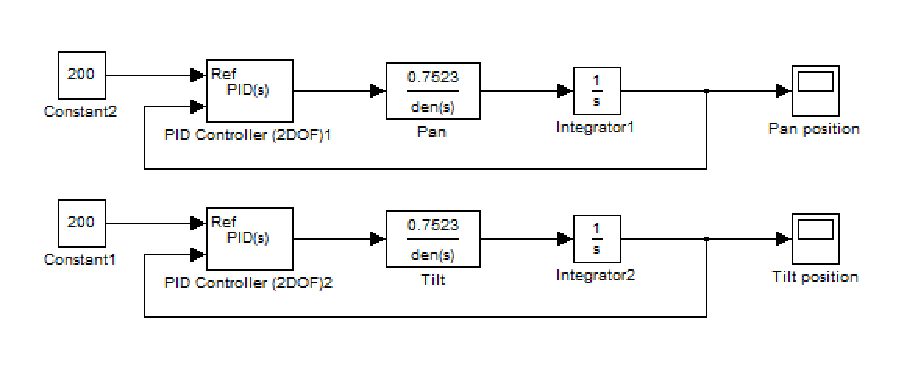
\includegraphics[width=\textwidth,trim=0 0 0 0]{graphics/Simulink.pdf} %trim=l b r t (can cut off from every side)
	\caption{This figure illustrates the simulink model.}
	\label{fig:control_simulink}			% figure labels are of the form \label{fig:*}
\end{figure}
The top system represent the pan part of the system, while the lower part represent the tilt.

\subsection{Simulation}
The goal of the simulation is to find the values providing a qickly responding system, while still remaining stable and robust. To obtain a first guess of the P-term, the root locus method is applied. The root locus plot can be seen in figure \ref{fig:rlocus_plot}. Aiming to minimize the energy needed to move the system, equal magnitudes of real and imaginary parts are chosen, leading to the base gain denoted in table \ref{tab:gain_values}.

\begin{figure}[htb]
	\centering
	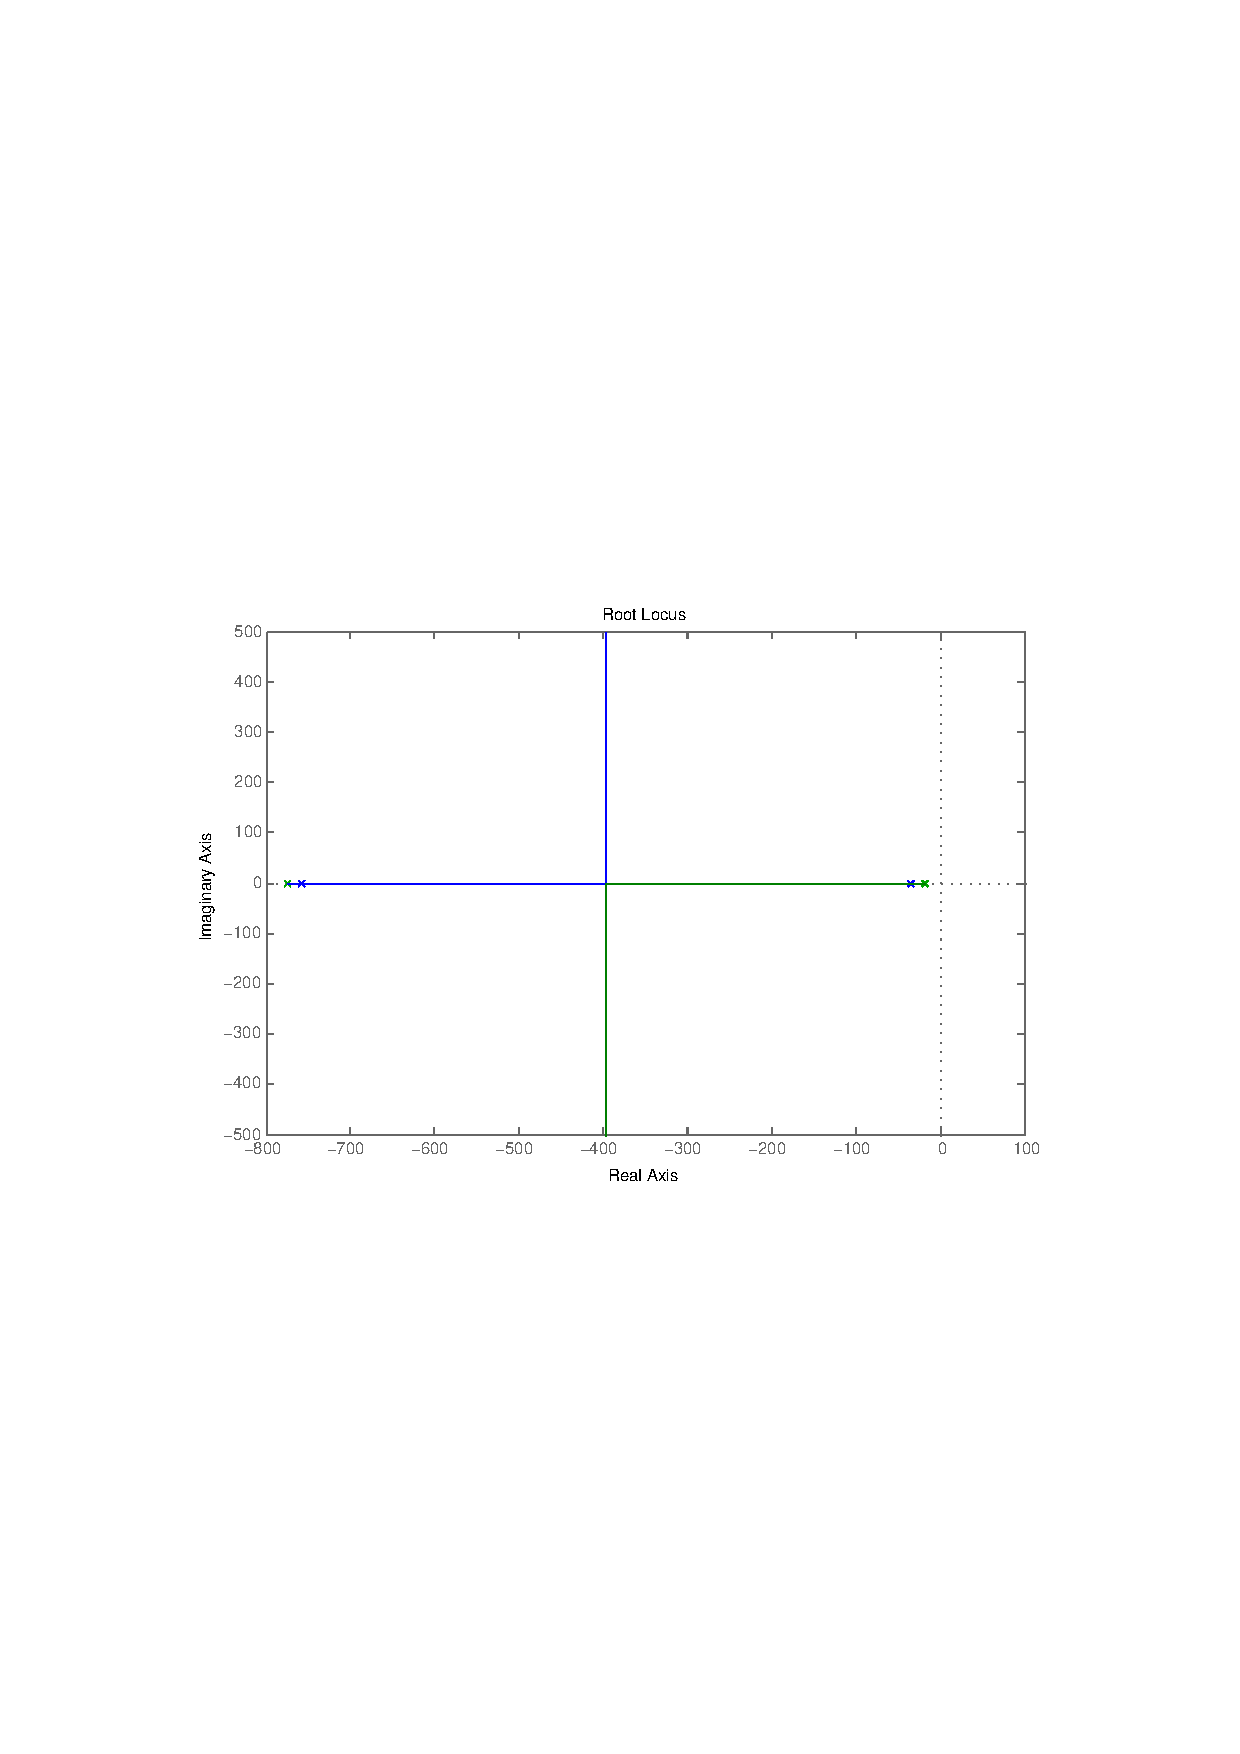
\includegraphics[width=\textwidth,trim=0 270 0 270]{graphics/rlocus_plot.pdf} %trim=l b r t (can cut off from every side)
	\caption{Shows the root locus plot the pan and tilt systems.}
	\label{fig:rlocus_plot}			
\end{figure}

The simulation is run with various parameters to find the range of values in table \ref{tab:gain_values}. Figure ??\marginnote{Undefined REF} shows a plot of the step response using autotuned parameters with response time 0,0175 s.

\begin{table}[htb]				
	\centering
	\begin{tabular}{lccc}			
	Term & Base & Maximum & Auto tune \\			
	\midrule												
P-gain pan& 6 & 450 & 145,87\\
P-gain tilt& 6 & 450 & 74,75 \\
I-gain pan& 0 & 250* & 315,36  \\
I-gain tilt& 0 & 350* & 160,79 \\
D-gain pan& 0 & 70** & 3,13 \\
D-gain tilt& 0 & 100** & 1,62\\
	\end{tabular}
	\caption{Gain values derived from simulation. *@P=30 and D=0. **@P=30 and I=0}				
	\label{tab:gain_values}			
\end{table}

\begin{figure}[htb]
	\centering
	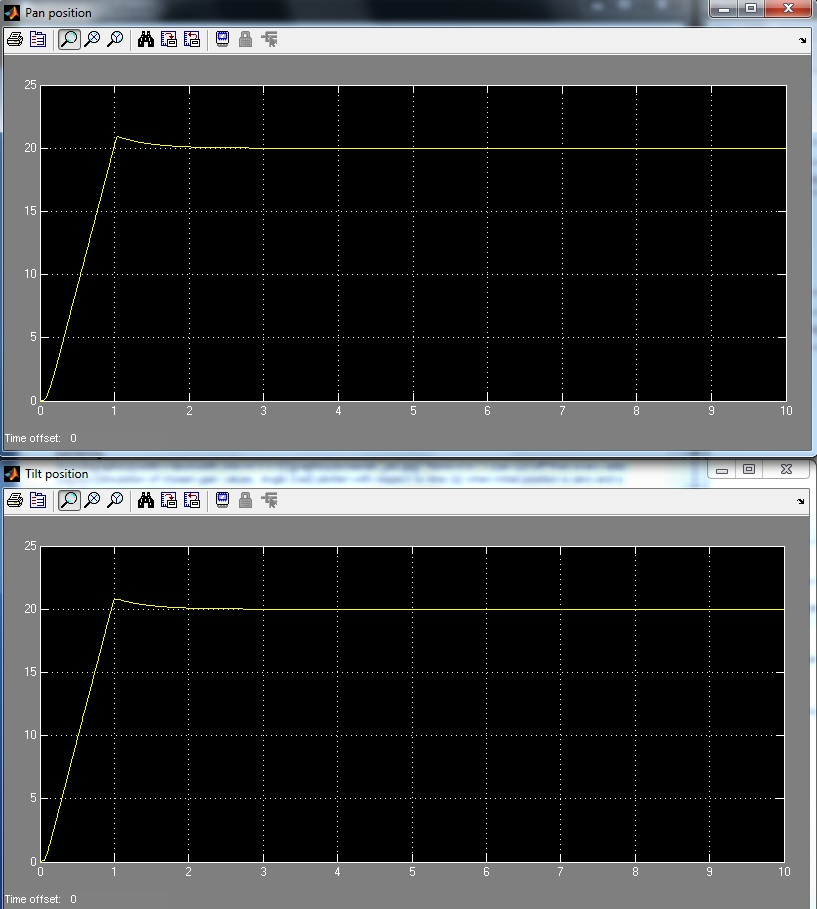
\includegraphics[width=\textwidth,trim=0 0 0 0]{graphics/screensh_pid.jpg} %trim=l b r t (can cut off from every side)
	\caption{Simulation of the autotune parameters. Angle[rad] plotted with respect to time[s] when initial position is zero and a setpoint of 20 is given as step.}
	\label{fig:chosen_plot}			% figure labels are of the form \label{fig:*}
\end{figure}

\subsection{Discussion}
The simulation of the was an easy and fast way of finding parameters for the PID regulator. Since the system has some limitations, this way of finding the range of parameters save the system from wear and tear. The autotune functionality of simulink and the ease of descretising the system also comes as credit for this approach.

In a regulator like this, there is a trade-off between having a dynamic fast responing system and having an accurate and smooth running system. In this case the objective was to obtain accuracy while remaining as dynamic system as possible.

\subsection{Conclusion}
The initial parameters for the PID regulator was found in an easy and safe way. The objective was to devolop a system able to track a position and with a steady state error of zero. Both of theese requrements were met, while keeping a faily dynamic system.

% START OF IMPLEMENTATION !!!!!!!!!!!!!!!!!!!!!!!!!!!!!!!!!!!!

\section{Implementation of PID control}
The control algorithm is implemented in the control task and all parameters are provided from the parameter server, but are cast as  floating point values for exact calculations.

When run the control task saves the value of the tick counter and when finished, it uses the FreeRTOS \texttt{vTaskDelayUntil} API to calculate when to unblock. As a starting point the control task runs at one hundred hertz frequency as verified in section \ref{subsec:control_freq}.

\begin{figure}[htb]
	\centering
	
\includegraphics[draft,width=\textwidth,trim=0 0 0 0]{blank}
	\caption{Shows a flowchart of the implemented control algorithm}
	\label{fig:pid_flow}			
\end{figure}

For calculating the error, a common format is needed. The parameter server holds the setpoint in degrees and the actual position in ticks. To be able to use some intuition about the control algorithm, degrees are chosen and the position in degrees is calculated by using a ticks to degrees factor calculated from knowing the gears and the number of ticks per motor round.
\begin{equation}
1 \ tilt \ revolution \ * 30:1 \ planet \ gear \ * 3:1 \ belt \ gear = 90 \ motor \ rounds
\end{equation}
\begin{equation}
 90 \ motor \ rounds * 12 \ ticks/round = 1080 \ ticks/tilt \ revolution
\end{equation}
This number is then used to calculate the ratio of degrees to ticks, keeping in mind that degrees have an implicit decimal:

\begin{equation}
\frac{360 \ deg \times 10}{1080 \ ticks} = 3.34\ deg/tick 
\end{equation}

The error is then calculated as the difference between setpoint and actual position and is thus a signed value in degrees.

To compare simulated values to actual values it is necessary to convert the gains so that \ref{eq:conv1} and \ref{eq:conv2} becomes equal. 
\begin{equation}
error \ [rad] * gain = input \ [V]
\label{eq:conv1}
\end{equation}
\begin{equation}
error \ [deg] * gain = input \ [pwm]
\label{eq:conv2}
\end{equation}

To convert from $rad$ to $deg$ the ratio is found
\begin{equation}
\frac{3600 \ deg}{2 \ \Pi \ rad} = 573 \ deg/rad
\label{eq:conv3}
\end{equation}
To convert from $[V]$ to $pwm$ the ratio is found
\begin{equation}
\frac{27.000 \ pwm}{12 \ V} = 2250 \ pwm/V
\label{eq:conv4}
\end{equation}
From equation \ref{eq:conv3} and \ref{eq:conv4} a conversion factor for the gain can be derived.
\begin{equation}
\frac{573}{2250} = 0,25
\label{eq:conv}
\end{equation}

\subsection{Implementing proportionality gain}
A first guess for the proportionality gain is to use the values provided by the autotune function in the simulation of the system. 

Since it is possible to get PWM values out of the range specified in table \ref{tab:parameters}, a maximum function is implemented, so that absolute values out of range are corrected to the maximum value.

Since PWM values below the minimum specified in table \ref{tab:parameters} does not make the motor move, a bias is added so that non-zero values are added with the bias value. This effectively narrows down the range of pwm signals to the value specified as actual pwm range in table \ref{tab:parameters}. 

A treshold is implemented so that values inside the +/- treshold area is zeroed before the bias is added. If this was not done even the smallest error would be biased.

Adjusting the P-gain is done empirically and is thus encompassed in section \ref{sec:pid_experiments_p}.

\subsection{Integrator}\label{sec:integrator}
As seen in section \ref{sec:pid_experiments_p} the system needs an integrator. Since the error grows smaller as the goal is approached, movement almost halt when approaching the goal area, making the system less accurate and slower. Therefore an integration term is implemented by adding the errror to the integration value on each run. Thereby in the situation where the error is too small to make the system move, the integration term will rise and thus add to the input. 

Normally an integration would mean the product of the value and the time since last sample, but presuming that this time is nearly constant it can be included in I-term. 

To keep the integration from going to infinity, an anti wind up filter is implemented. Wind up happens for example when the system is stopped while not at the setpoint and the integration reaches high values that has to be overcome when the system resumes.

As with the P-gain, adjusting the I-gain is done empirically and is thus encompassed in section \ref{sec:pid_experiments_i}.

\subsection{Differentiator}
By saving the error at each entry it is possible to calculate the change in the error. This term will be particularly large just after changing the setpoint, and can thus help improve the acceleration. 

The actual derivative would be the change in value over the time since last entry, but as for the integrator, this can be omitted presuming that it is constant. Since the point is to oppose the changes, the D-term of the pwm calculation is subtracted to keep the gain a positive value.

As with the P- and I-gain, adjusting the D-gain is done empirically and is thus encompassed in section \ref{sec:pid_experiments_i}


\subsection{Discussion}
The implemented PID regulator performs very well as seen from \ref{sec:precisionofsystem2} and the performance is almost at the theoretical limit with respect to precision. More could be done in terms of speed and setting time, but it could not be improved without knowing the explicit purpose of the system and further refinement is thus outside the scope of this project.

\subsection{Conclusion}
The decision to abandon the full state feedback regulator has been proved right, since optimal results were obtained by using a much simpler approach. Though the implemented regulator is somewhat rough, it works well and provides a base for further development.











